\chapter{Trabalhos relacionados}
\label{chapter:relacionados}

No motor de pesquisa acadêmica Google Scholar foram feitas pesquisas associando as áreas de conhecimento de desenvolvimento de nanossatélites, testes de software e automação de testes. As pesquisas foram realizadas ao longo da elaboração do trabalho e diferentes \textit{strings} de busca foram utilizadas. Como critério para escolha das publicações à serem estudadas, foram analisados os resultados apresentados na primeira página do motor de busca. Para determinar a relevância de uma publicação para o trabalho, foi analisado o \textit{abstract} e a introdução dos mesmos. Para os trabalhos relacionados apresentados neste capítulo os resultados e conclusõestambém foram estudados.


\begin{quadro}[h!]
\caption{Pesquisas realizadas}
\begin{tabular}{|l|l|}
\hline
\textit{String}          & Resultados \\ \hline
software+reliabilty+test & 565,000    \\
nanosattelite + design   & 15,200     \\
software + test          & 4,300,000  \\
software+test+automation & 1,970,000  \\
flatsat + cubesat        & 359        \\
cubesat                  & 29,200     \\
flatsat + nanosatellite  & 273        \\
cubesat + testbed        & 3,510      \\ \hline
\end{tabular}
 \label{quadro:pesquisas}
 \legend{Fonte: Autor.}
\end{quadro}

\section{Software Reliability Growth With Test Coverage \texorpdfstring{\cite{malaiya-2002}}{} }
\label{relacionados:malaiya-2002}
O termo "cobertura de testes", do inglês \textit{test coverage} quantifica o grau de rigor dos testes. Existem ferramentas que são capazes de mensurar a cobertura de testes em diferentes termos, como \textit{branches}, e inteção de uso. Os autores deste artigo trazem uma relação entre duração dos testes, cobertura e confiabilidade de software.

Desenvolvedores são capazes de atingir o nível de confiabilidade de \textit{software} de maneira previsível a partir de análise de confiabilidade durante o desenvolvimento. Para quantificar essa métrica durante os testes, o código é executado com \textit{inputs} selecionados aleatoriamente seguindo uma distribuição determinada. Dessa forma, se a distribuição utilizada for a mesma esperada durante a vida operacional do \textit{software}, pode ser levantado um modelo de confiabilidade a partir dos resultados dos testes.

Os autores constatam, no entanto, que para focar os testes na detecção de erros, é mais produtivo executar o código com \textit{inputs} considerados especialmente para estimular comportamentos onde erros são mais prováveis, e propõem neste estudo um modelo para realizar essa mensuração. Dentre os resultados obtidos na análise, os autores constatam que  em muitos casos, um mínimo de 85\% de cobertura de testes é necessário para aumento significativo na confiabilidade do software em desenvolvimento.

\section{How Do Software Developers Use GitHub Actions
to Automate Their Workflows? \texorpdfstring{\cite{kinsman-2021}}{} }
\label{relacionados:kinsman-2021}
Ferramentas sociais de programação, como o GitHub, alteraram a natureza colaborativa de desenvolvimento de \textit{software open source}, proporcionando novas oportunidades para engajamento, mas ao mesmo tempo aumentando a carga de trabalho de mantenedores de repositórios, que devem revisar, comunicar, explicar o projeto e gerenciar o versionamento de um número muito maior de colaboradores.

Para reduzir essa carga de trabalho intensiva, os autores estudam a ferramenta GitHub Actions, disponibilizada em 2019, que permite aos usuários automatizar questões como verificar se o código compila, se todos os testes são executados com sucesso, ou ainda se o código está dentro dos padrões de desenvolvimento do projeto. Esse controle pode ser feito segundo diversos \textit{triggers}, como \textit{commits}, comentários, \textit{issues} ou \textit{pull-requests}.

No artigo, os autores estudaram como desenvolvedores de software fazem uso da ferramenta para automatizar os fluxos de trabalho, como a ferramenta é discutida, e quais seus efeitos nos \textit{pull requests} dos projetos. Com uma amostra de 3,190 repositórios ativos no GitHub, e análise estatística de 926 deles, foi constatado que apenas uma pequena parcela dos repositórios utiliza a ferramenta, mas que a plataforma é vista, em geral, como benéfica para os contribuidores. Entre esses repositórios, os autores encontraram 708 \textit{workflows} de automação únicos.

Os autores relatam também que a utilização da ferramenta acarretou em diminuição da quantidade de aprovação de \textit{commits} mensal, e aumentou a quantidade de \textit{pull requests} rejeitados, experiências anedóticas revelam que a ferramenta e as funcionalidades que ela apresenta são recebidas com entusiasmo e apreciação pelos desenvolvedores.


\section{An Architecture-Tracking Approach to Evaluate
a Modular and Extensible Flight Software
for CubeSat Nanosatellites \texorpdfstring{\cite{gonzales-2019}}{}}
\label{relacionados:gonzales-2019}
Um ponto importante para aumentar o sucesso de missões CubeSat é a entrega de \textit{software} de vôo de qualidade. Esse tópico é identificado como chave para elevar a qualidade de diversos pontos de uma missão, como reusabilidade, colaboração, redução de riscos e facilitação de desenvolvimento. Uma arquitetura \textit{software} de vôo apropriada representa  os requisitos funcionais e não funcionais e guia o desenvolvimento. Dessa forma, para atingir o nível de qualidade desejada a arquitetura deve ser monitorada durante todo o ciclo de desenvolvimento de \textit{software}. Esse monitoramento, no entanto, é difícil e não-trivial.

Neste artigo, Gonzales \textit{et al.} apresentam detalhes sobre a implementação de missões CubeSat que se mostraram bastante similares à metodologia empregada no desenvolvimento do FloripaSat-2. Os autores trazem em seu trabalho pontos importanes sobre como entregar software de qualidade, confiável etolerante a falhas para missões CubeSat, que como toda missão espacial, se tratam de sistemas críticos que de modo geral devem operar de maneira autônoma e cujo software e hardware não podem ser corrigidos após o lançamento.

Os pontos de maior relevância para este trabalho são os requisitos não-funcionais de uma missão CubeSat trazidos pelos autores, entre eles a confiabilidade e extensibilidade do código, e a metodologia de projeto e arquitetura do \textit{software} de vôo, como a distinção entre as camadas do sistema, utilização de repositórios e em especial os métodos de validação utilizando métodos de integração contínua como ferramenta para elevar a confiabilidade do sistema através de testes automatizados.

Os temas apresentados pelos autores serão discutidos de forma mais profunda na \autoref{proposta:confiabilidade} e \autoref{projeto:floripasat2}.

\section{Integration and Verification Approach of ISTSat-1 CubeSat \texorpdfstring{\\ \cite{aiv-cubesat}}{} }
\label{relacionados:aiv-cubesat}
Satélites artificiais precisam resistir a uma grande quantidade de adversidades enquanto operam em um ambiente hostil e inóspito. Por isso é essencial que sejam feitos testes extensivos para garantir o nível de confiança necessário para que o objetivos da missão sejam atingidos. Porém, missões de CubeSat tendem a não ser tão rigorosas em suas etapas de montagem, integração e verificação (AIV), fato que é refletido na taxa de missões que acabam em falhas.

Esse paradigma, no entanto, está mudando a medida que a importância do CubeSats aumenta. Ela vai de simplesmente projetos educacionais, para missões de custos e importância elevados. Um exemplo desse salto é a missão Mars Cube One, ou MarCO \cite{mars-cubesat}, desenvolvida pelo \textit{Jet Propulsion Laboratory} da Nasa, que enviou dois CubeSats a Marte, para servirem como satélites de comunicação. Assim, os autores desse artigo apresentam a ideia de que integração e verificação em missões CUbeSats passam a ser encaradas com mais seriedade, como demonstrado na figura \ref{fig:nanosats_years_forecast}, onde é possível observar o aumento de lançamento de nanossatélites e, paralelamente, a diminuição da taxa de falhas.

Como estudo de caso, o artigo apresenta o processo de AIV empregado no desenvolvimento do ISTSat-1 \cite{istsat-1}, o primeiro nanossatélite português, lançado em 2021 e que utilizou a estratégia de teste através de uma \textit{FlatSat}, que se trata de uma plataforma de testes de \textit{Hardware In the Loop} (HIL).

A equipe do ISTSat-1, segundo os autores, optou por desenvolver a maioria dos subsistemas do satélite e adotou métodos ágeis para as atividades de AIV de forma a diminuir os riscos relacionados a falta de experiência da equipe. Dessa forma foi possível desenvolver e testar os módulos de forma contínua e iterativa, o que possibilitou a descoberta rápida de diversos erros e problemas que necessitavam de ajustes de design. Foi concluído nesse estudo que, caso a equipe tivesse optado por um processo de desenvolvimento em cascata, como tradicionalmente empregado em missões CubeSat, seria mais difícil, senão impossível, ter descoberto os mesmos problemas no design e funcionamento. Concluem então, que a adoção de processos iterativos é útil para projetos educacionais que contam com equipes sem muita experiência, ou sem muitos recursos financeiros.

\begin{figure}[h!]
    \centering
    \caption{Lançamentos anuais de Nanossatélites (previsão)}
    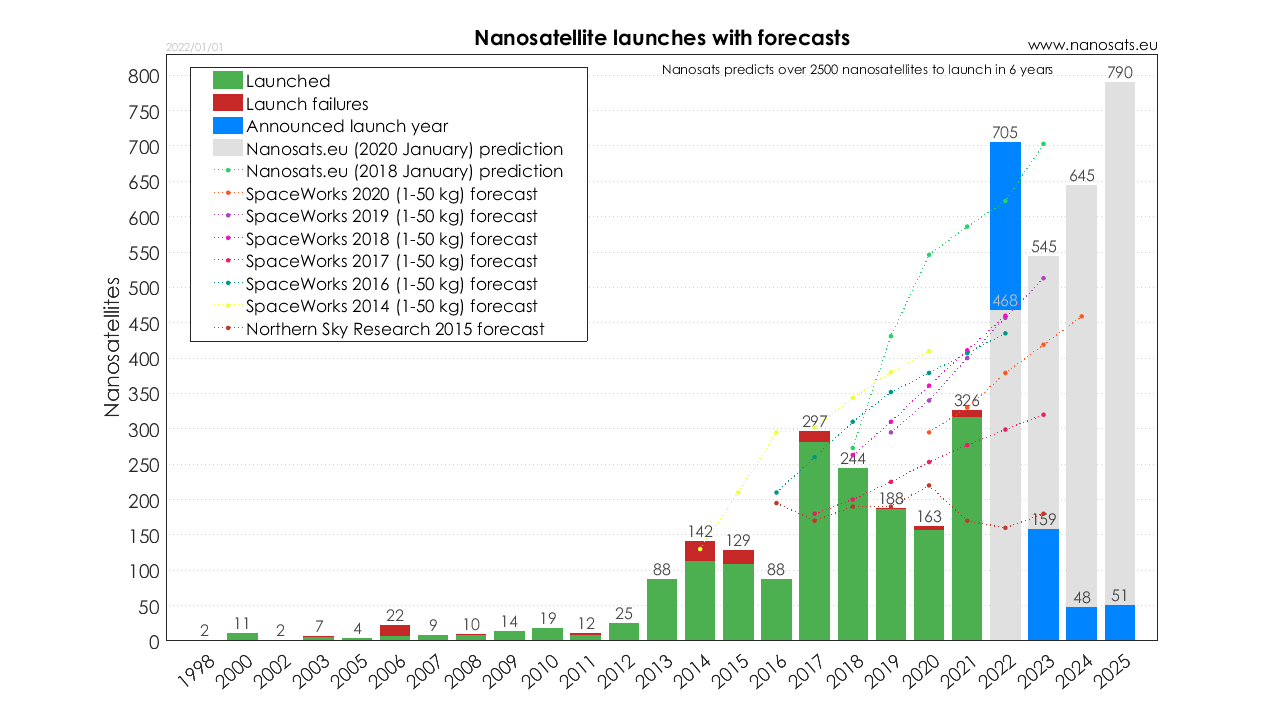
\includegraphics[width=\textwidth]{images/nanosat_years_forecast.png}
    \legend{Fonte: Nanosats Database \cite{nanosats-database}}
    \label{fig:nanosats_years_forecast}
\end{figure}


\section{Qualification and validation test methodology of the open-source CubeSat FloripaSat-I \texorpdfstring{\cite{marcelino2020-2}}{} }
\label{relacionados:marcelino2020-2}
Esta seção e a próxima apresentam dois trabalhos produzidos como resultado da missão FloripaSat-1, uma missão de demonstração desenvolvida inteiramente por estudantes da Universidade Federal de Santa Catarina (UFSC), cujo CubeSat foi lançado em 2019.

O FloripaSat-1 é composto de três módulos distintos, o sistema elétrico - EPS (\textit{Electric Power System}), o módulo de gerência de dados - OBDH (\textit{Onboard Data Handling}) e o módulo de telemetria e telecomandos - TT\&C (\textit{Telemetry, Tracking and Command}).

O artigo informa que a missão tinha como objetivo testar tecnologias que possibilitem o desenvolvimento rápido e de baixo custo de satélites espaciais, além de treinar estudantes nas áreas de concepção, implementação e operação de uma missão espacial completa. Além disso, o FloripaSat-1 é um projeto \textit{open source} e as informações de software e hardware dos módulos desenvolvidos estão disponíveis em repositórios públicos, para uso em futuras missões.

Os autores descrevem que o FloripaSat-1 foi desenvolvido com base em projetos de engenharia de sistemas, dividido em Modelos de protótipo (PM), engenharia (EM-I e EM-II) e finalmente o Modelo de Vôo (FM). Foram realizados testes em cada uma dessas etapas para validar os sistemas e os resultados, segundo o artigo, foram decisivos na detecção e correção de erros.

Apesar do artigo focar em integração e validação dos módulos a nível de hardware, julga-se relevante para a elaboração deste trabalho, que foca principalmente em software, por descrever as diferentes condições que uma missão espacial é submetida, além da metodologia de desenvolvimento adotada pela equipe do FloripaSat-1, em que a grande maioria dos membros seguiu para a missão FloripaSat-2, a qual este trabalho se baseia.

\section{A Critical Embedded System Challenge: The FloripaSat-1 Mission \texorpdfstring{\\\cite{marcelino2020-1}}{} }
\label{relacionados:marcelino2020-1}
Este artigo, elaborado também a partir da missão FloripaSat-1 do SpaceLab, apresenta definições e descrições dos subsistemas do satélite, além de algumas informações e resultados de testes e simulações realizadas nos mesmos.

Como descrito anteriormente, o FloripaSat-1 possui três sub sistemas principais:

\begin{itemize}
    \item \textit{Electric Power System} (EPS)
    \item \textit{On-Board Data Handling} (OBDH)
    \item \textit{Tracking, Telemetry and Command} (TT\&C)
\end{itemize}

O EPS é o módulo responsável por distribuir, coletar e armazenar a energia utilizada pelo satélite. A energia é coletada através de painéis solares e armazenada em uma bateria de íon de lítio. A distribuição da energia é definida a partir de um microcontrolador que analisa os estados de carga e de energia e decide quais módulos permanecerão em operação.

O OBDH é o módulo responsável pela gerência de atividades do satélite. Ele realiza a interface entre todos os subsistemas do satélite. Os dados gerados são empacotados e transmitidos através do TT\&C, e dados recebidos são enviados ao OBDH para que ele execute a tarefa requisitada, ou então envie o comando ao módulo requisitado. Este módulo também possui uma memória, para que possam ser futuramente recuperados.

Finalmente, o TT\&C é o módulo responsável pela comunicação entre o satélite e as estações de controle na Terra. Ele opera através de dois módulos de rádio, um para a banda VHF e um para UHF. Os comandos a serem enviados e recebidos pelo satélite (\textit{downlink}/ \textit{uplink}) são transmitidos através do módulo UHF e a banda VHF é reservada para transmissões do tipo \textit{beacon}.

Os autores discorrem ainda sobre os demais módulos e subsistemas do satélite, como outros \textit{payloads} que não foram desenvolvidos ou projetados pela equipe da UFSC e portanto, ficam de fora desse breve resumo.

A relevância deste artigo se dá pelo fato de que o FloripaSat-2 utiliza a mesma estrutura de subsistemas, com os seus módulos sendo sucessores diretos do software e hardware utilizados na missão anterior, operando de forma idêntica ou muito similar.


\section{In-orbit preliminary results from the open-source educational nanosatellite FloripaSat-I \texorpdfstring{\\\cite{marcelino2021}}{} }
\label{relacionados:marcelino2021}
O FloripaSat-I, como mencionado anteriormente, constituiu uma missão CubeSat desenvolvida na Universidade Federal de Santa Catarina, em que os objetivos incluiam testar tecnologias que permitissem desenvolvimento mais rápido e menos custoso de satélites futuros através do reuso da estrutura \textit{open source}. Lançado em 2019 em um foguete Chinês Long March 4B, os dados transmitidos pelo satélite foram usados como métricas de validação da missão, permitindo aos desenvolvedores (em sua maioria estudantes da UFSC) traçar paralelos entre os dados de órbita e as análises obtidas em laboratório.

Os autores apresentam uma análise dos resultados coletados durante os primeiros três meses da missão, além das lições aprendidas através dos dados recebidos.

O FloripaSat-I foi lançado em uma órbita heliossíncrona, que se trata de uma configuração de órbita quase polar, onde o plano de órbita é sempre fixo em relação ao Sol, e o objeto em órbita passa pela sobre a mesma região da superfície no mesmo instante todos os dias.\cite{tscherbakova-1998}.

Os dados enviados pelo satélite foram coletados em múltipas estações espalhadas pelo mundo, como apresentado na figura \autoref{fig:floripasat-stations}, e decodificados através de um \textit{software} de estação terrestre desenvolvido no laboratório.

\begin{figure}[h!]
    \centering
    \caption{Estações que receberam dados enviados pelo FloripaSat-I nos três primeiros meses da missão.}
    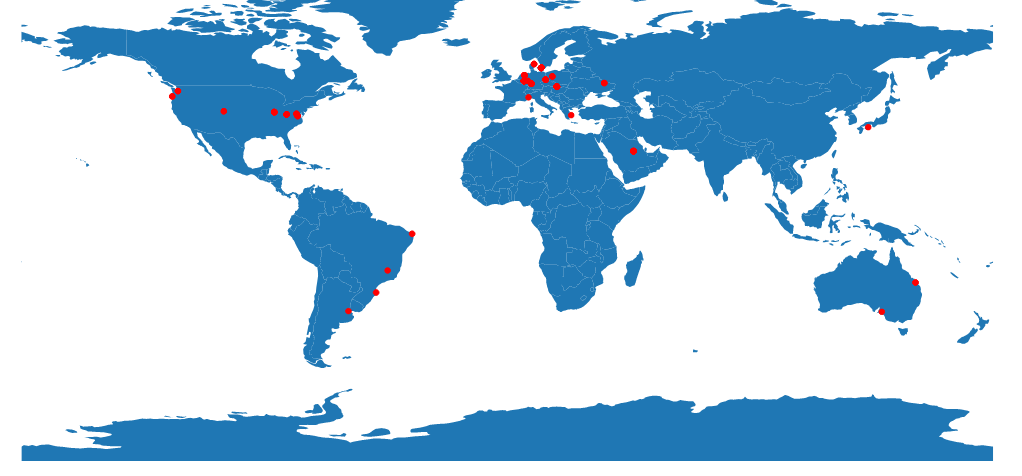
\includegraphics[width=\textwidth]{images/floripasat_stations.png}
    \legend{Fonte: \cite{marcelino2021}}
    \label{fig:floripasat-stations}
\end{figure}

No estudo publicado, os autores elencam algumas das dificuldades encontradas durante o desenvolvimento da missão e reveladas pelos dados do satélite em órbita, em especial dificuldades na montagem, que pode ter acarretado em problemas estruturais e de funcionamento, e de frequências utilizadas, que dificultaram a comunicação.

Além disso, foi realizada uma análise com os participantes do projeto com o intuito de compreender como a missão os afetou, e os resultados obtidos foram em geral percebidos como positivos pelos estudantes, que reportaram não apenas evolução de aprendizado e de experiência de desenvolvimento.

%

\section{Considerações}

Os artigos e teses escolhidos para embasar e fundamentar este trabalho estabelecem a importância de um modelo de testes bem estruturado em um projeto de desenvolvimento de \textit{software}. Todos os trabalhos relacionados a missões CubeSat mencionam a importância dos testes para a descoberta e solução de erros, bem como a relação entre a execução e planejamento dos testes e o aumento de confiabilidade do \textit{software.}, como demonstrado pelo estudo apresentado na \autoref{relacionados:malaiya-2002}.

O artigo apresentado na \autoref{relacionados:gonzales-2019} é especialmente interessante para a proposta desse trabalho por descrever em detalhes o processo e as práticas de desenvolvimento aplicadas na série de nanossatélites \textit{SUCHAI}, que se assemelham ao modelo proposto neste trabalho. Os autores citam diversos modelos e práticas de desenvolvimento que são, em essência, seguidos de maneira muito próxima pela missão FloripaSat-II, como será evidenciado no \autoref{chapter:proposta} e \autoref{chapter:projeto}.

O artigo analisado na \autoref{relacionados:marcelino2021}, apresenta uma análise dos resultados obtidos nos meses iniciais de operação do FloripaSat-I, bem como uma análise do impacto do satélite nos estudantes envolvidos no projeto. Este artigo demonstra as dificuldades encontradas no desenvolvimento da missão, e servem o propósito de indicar pontos de atenção e melhoria para trabalhos futuros, como é o caso do FloripaSat-II, que se inspira e por vezes diretamente reimplementa os sistemas utilizados no seu antecessor.

Além disso, os outros dois trabalhos produzidos por membros do SpaceLab, descritos na \autoref{relacionados:marcelino2020-1} e \autoref{relacionados:marcelino2020-2}, que relatam o processo de desenvolvimento da missão FloripaSat-1 mostram a importância de CubeSats como ferramenta educacional, servindo para treinar e capacitar estudantes no projeto, desenvolvimento e operação de uma missão espacial completa.

O modelo proposto por este trabalho é, então, uma continuidade dos pensamentos apresentados neste capítulo. Espera-se que o sistema implementado permita aumentar a qualidade e a confiabilidade do código entregue através de técnicas de integração contínua para automatizar os testes de unidade dos sistemas embarcados desenvolvidos para o FloripaSat-II, além de possibilitar mais uma ferramenta com potencial de estudo e aprendizado, sob a qual podem ser empregadas futuras ferramentas para analisar e expandir o modelo, como detalhado na \autoref{conclusao:futuros}.

\iffalse

\fi